\let\lesson\undefined
\newcommand{\lesson}{\phantomlesson{Bài 13: Một số ví dụ về cách giải các bài toán thuộc phần động lực học}}
\chapter[Một số ví dụ về cách giải các bài toán thuộc phần động lực học]{Một số ví dụ về cách giải các bài toán thuộc phần động lực học}
\setcounter{section}{0}
\section{Phương pháp chung}

Phương pháp phân tích lực giải bài toán động lực học là phương pháp khảo sát chuyển động của các vật dựa trên cơ sở các định luật Newton. Phương pháp phân tích lực bao gồm các bước cơ bản sau:
\begin{enumerate}[label=\textbf{\arabic*}.]
	\item \textbf{Xác định các lực tác dụng lên vật hoặc hệ vật và vẽ giản đồ lực.}
	
	Các lực cần được xác định rõ điểm đặt, phương, chiều, độ lớn. Các lực thường gặp là: 
	\begin{itemize}
		\item Các lực do các trường lực gây ra như trường hấp dẫn, điện trường, từ trường, $\ldots$
		\item Các lực do liên kết giữa các vật trong hệ: lực căng dây, lực đàn hồi, $\ldots$
		\item Các lực do tiếp xúc giữa vật và các vật khác: áp lực, phản lực, lực ma sát.
	\end{itemize}
	\item \textbf{Viết phương trình định luật II Newton cho vật hoặc hệ vật }
	
	Phương trình viết ở dạng vectơ 
	\begin{align}
		\sum\vec{F}=m\vec{a},
	\end{align}
	trong đó $\sum\vec{F}$ là tổng vectơ các lực tác dụng lên vật hoặc hệ vật, $m$ là khối lượng của vật hoặc hệ vật tương ứng. 
	
	Trong trường hợp hệ gồm nhiều vật, ứng với mỗi vật có thể viết một phương trình định luật II Newton tương ứng
	$$\begin{cases}
		m_1 \vec{a}_1 = \Sigma \vec{F}_1\\
		m_2 \vec{a}_2 = \Sigma \vec{F}_2\\
		\ldots\\
		m_n \vec{a}_n = \Sigma \vec{F}_n\\
	\end{cases}$$
	trong đó  $\Sigma \vec{F}_n$ là tổng các lực tác dụng vào vật thứ $n$, $m_n$ là khối lượng của vật thứ $n$ tương ứng. 
	
	\item \textbf{Giải phương trình định luật II Newton }
	
	Phương trình định luật II Newton là phương trình vectơ. Một trong những cách phổ biến để giải phương trình này là chiếu phương trình này lên các trục tọa độ và giải hệ các phương trình hình chiếu. 
	
	Đối với các bài hệ vật, ta có thể chọn một hệ trục chung cho cả hệ, hoặc ứng với mỗi vật lại chọn một hệ trục riêng. Khi đó mỗi phương trình định luật II Newton ứng với mỗi vật cần phải được chiếu lên hệ trục tương ứng. Ngoài ra ta cũng cần xác định rõ mối liên hệ gia tốc giữa các vật trong hệ, thường được xác định qua liên hệ tọa độ các vật. 
\end{enumerate}

\manatip{Phản lực $\vec{N}$ luôn vuông góc với mặt tiếp xúc, còn lực ma sát luôn có phương tiếp tuyến mặt tiếp xúc, nên ta thường chọn hệ trục O$xy$ có trục O$y$ vuông góc mặt tiếp xúc, O$x$ song song mặt tiếp xúc. Như vậy, phương trình hình chiếu định luật II Newton trên trục O$y$ cho phép ta xác định được biểu thức của phản lực $N$. Thay biểu thức này vào lực ma sát $F_\text{ms}=\mu N$ trong phương trình hình chiếu trên trục O$x$ sẽ giúp ta giải được bài toán.}

\section{Mục tiêu bài học - Ví dụ minh hoạ}
\begin{dang}{Phương pháp động lực học cho bài toán chuyển động của một vật}
	\ppgiai{Để giải bài toán động lực học cho chuyển động của một vật, các em thực hiện các bước như sau:
		\begin{itemize}
			\item \textbf{Bước 1:} Chọn vật khảo sát chuyển động. Biểu diễn các lực tác dụng lên vật, trong đó làm rõ phương, chiều và điểm đặt của từng lực.
			\item \textbf{Bước 2:} Viết phương trình định luật II Newton
			$$\overrightarrow{F_1}+\overrightarrow{F_2}+\dots+\overrightarrow{F_n}=m\vec{a}.$$
			\item \textbf{Bước 3:} Chọn hệ trục toạ độ vuông góc $Oxy$; trong đó $Ox$ cùng hướng với hướng chuyển động của vật hay cùng hướng với lực kéo khi vật đứng yên. Phân tích các lực theo hai trục này. Chiếu phương trình định luật II Newton lên hai trục $Ox$ và $Oy$
				$$\begin{cases}
					Ox: F_x=F_{1x}+F_{2x}+\dots+F_{nx}=m\cdot a_x \\
					Oy: F_y=F_{1y}+F_{2y}+\dots+F_{ny}=m\cdot a_y
				\end{cases}$$
			\item \textbf{Bước 4:} Giải hệ phương trình tren ta tìm được gia tốc chuyển động hay lực tác dụng, tuỳ từng bài toán.
		\end{itemize}
}
\viduii{3}{
	Một vật nhỏ khối lượng $m$ chuyển động theo trục O$x$ trên mặt phẳng nằm ngang dưới tác dụng của lực kéo $\vec F$ chếch lên theo hướng hợp với O$x$ một góc $\alpha>0$. Hệ số ma sát trượt trên mặt ngang bằng $\mu_\text{t}$. Xác định gia tốc chuyển động của vật
}
{\hide{
	\begin{center}
		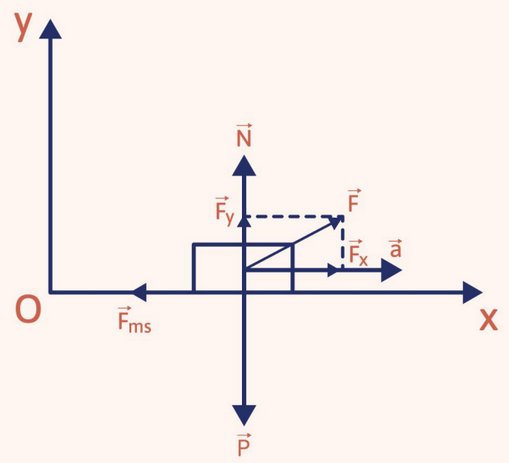
\includegraphics[scale=0.5]{../figs/G10-17-1}
	\end{center}
	
	\begin{itemize}
		\item Các lực tác dụng lên vật gồm lực kéo $\vec F$, lực ma sát $\vec F_\text{ms}$, trong lực $\vec P$, phản lực $\vec N$ được thể hiện trên giản đồ. 
		
		\item Phương trình định luật II Newton có dạng 
		\begin{equation}\label{*}
			\vec F +\vec F_\text{ms} + \vec P + \vec N = m \vec a
		\end{equation}
		
		\item Chọn hệ trục tọa độ: O$x$ nằm ngang, O$y$ thẳng đứng hướng lên trên và chiếu phương trình \eqref{*} lên các trục tọa độ đã chọn:
		\begin{itemize}
			\item Chiếu (\ref{*}) lên O$y$:
			\begin{equation}\label{***}
				F_y + N - P = 0 \\
				\quad\Rightarrow\quad N = P - F\sin \alpha
			\end{equation}
			\item Chiếu ($\ref{*}$) lên O$x$:
			\begin{equation}\label{**}
				F_x - F_\text{ms} = ma \\
				\quad\Rightarrow\quad F \cos \alpha - \mu_\text{t} N = ma
			\end{equation}
		\end{itemize}
		Thay $N = P - \sin \alpha$ từ phương trình \eqref{***} vào phương trình \eqref{**}, ta tính được 
		$$a=\dfrac{F \cos \alpha - \mu_\text{t} (P-F\sin \alpha)}{m}.$$
	\end{itemize}
}}


\viduii{3}{
	Một chiếc hộp gỗ được thả trượt không vận tốc ban đầu, từ đầu trên của một tấm gỗ dài $L=\SI{2}{m}$. Tấm gỗ đặt nghiêng $30^\circ$ so với phương ngang. Hệ số ma sát giữa đáy hộp và mặt gỗ là $\SI{0.2}{}$. Lấy $g=\SI{9.8}{m/s^2}$. Hỏi sau bao lâu thì hộp trượt xuống đến đầu dưới của tấm gỗ?
}
{\hide{
	\begin{center}
		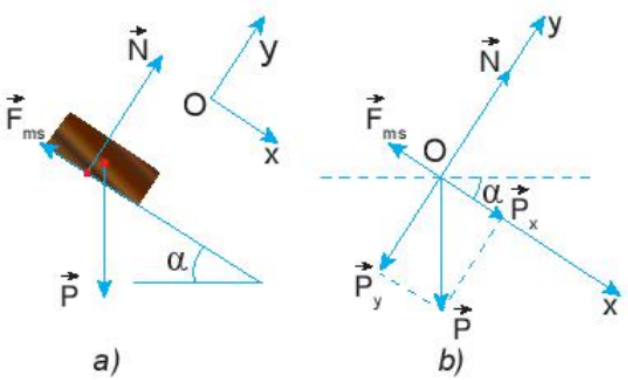
\includegraphics[scale=0.5]{../figs/G10-17-3}
	\end{center}
	
	\begin{itemize}
		\item Hộp gỗ (coi là chất điểm) chịu tác dụng của ba lực: trọng lực $\vec P$, phản lực $\vec N$ và lực ma sát $\vec F_\text{ms}$ như ở hình bên trái.
		
		\item Phương trình định luật II Niu-tơn:
		\begin{equation}\label{10}
			\vec F_\text{ms} + \vec P + \vec N = m \vec a
		\end{equation}
		
		\item Chọn hệ trục tọa độ: O$x$, O$y$ như hình vẽ. Phân tích trọng lực $\vec P$ thành hai lực thành phần $\vec P_x$, $\vec P_y$ như trong hình bên phải.
		
		Chiếu các vectơ lực lên các trục tọa độ đã chọn:
		\begin{itemize}
			\item Chiếu (\ref{10}) lên O$y$:
			\begin{equation}\label{12}
				N - mg \cos \alpha = 0 \quad\Rightarrow N = mg\cos\alpha \quad\Rightarrow F_\text{ms}=\mu N=\mu mg \cos\alpha.
			\end{equation}
			\item Chiếu ($\ref{10}$) lên O$x$:
			\begin{equation}\label{11}
				mg \sin \alpha - F_\text{ms} = ma \quad\Rightarrow a= g(\sin \alpha - \mu \cos \alpha)
			\end{equation}
		\end{itemize}
		
		Thay số, ta được $a \approx \SI{3.2}{\meter/\second}$. Vậy hộp trượt xuống với gia tốc $a=\SI{3.2}{\meter/\second^2}$, cùng chiều với trục O$x$.
		
		\item Áp dụng công thức xác định thời gian trong chuyển động thẳng biến đổi đều:
		$$L=\dfrac{1}{2}at^2\quad\Rightarrow\quad t=\sqrt{\dfrac{2L}{a}} \approx \SI{1.1}{\second}$$
	\end{itemize}
}}
\end{dang}
\begin{dang}{Giải bài toán hệ vật liên kết dây bằng việc phân tích chuyển động của từng vật}
	\ppgiai{Để giải các bài toán liên quan đến chuyển động của hệ vật liên kết dây, các em thực hiện các bước giải như sau:
	\begin{enumerate}[label=\bfseries Bước \arabic*.]
		\item Phân tích các lực tác dụng lên mỗi vật.
		\item Viết phương trình định luật II Newton cho mỗi vật.
		\item Chọn hệ trục toạ độ $Oxy$. Chiếu phương trình định luật II Newton của mỗi vật lên các phương $Ox$ và $Oy$.
		\item \begin{itemize}
			\item Nếu dây không dãn thì quãng đường mỗi vật chuyển động là như nhau $\Rightarrow a_1=a_2$.
			\item Nếu bỏ qua khối lượng của dây, khối lượng và bán kính của ròng rọc thì lực căng tại mỗi điểm trên dây là như nhau $T_1=T_2$.
		\end{itemize}
	\item Giải hệ phương trình động lực học trên ta tìm được các đại lượng đề bài yêu cầu.
	\end{enumerate}
}
\viduii{4}{Hai vật 1 và 2 có thể trượt trên mặt bàn nằm ngang và được nối với nhau bằng dây không dãn, khối lượng dây không đáng kể. Khối lượng của các vật là $m_1 = \SI{2}{kg}$, $m_2=\SI{1}{kg}$. Tác dụng vào vật 1 lực $F=\SI{9}{N}$ theo phương song song với mặt bàn. Hệ số ma sát giữa hai vật với mặt bàn là $\mu=\SI{0.2}{}$. Lấy $g=\SI{10}{m/s^2}$. Hãy tính gia tốc chuyển động của các vật.
}
{\hide{
	\begin{center}
		\begin{tikzpicture}
			\node[anchor=south west,inner sep=0] at (0,0) {\includegraphics[scale=0.7]{G10-17-2}};
			\draw[red,thick,-stealth] (6.8,1.35) -- (5.9,1.35);
			\node[below] at (5.9,1.35) {$\vec{\text{F}}_{\text{ms}_1}$};
		\end{tikzpicture}
		%	\includegraphics[scale=0.5]{../figs/G10-17-2}
	\end{center}
	
	\begin{itemize}
		\item Đối với vật 1:
		\begin{equation}\label{1}
			\vec P_1 + \vec N_1 + \vec T_1 + \vec F_\text{ms1} + \vec F = m_1 \vec a_1
		\end{equation}
		
		Chiếu (\ref{1}) xuống O$x$: $F - T_1 - F_\text{ms1} = m_1 a_1$.
		
		Chiếu (\ref{1}) xuống O$y$: $-m_1 g + N_1 = 0$.
		
		Với $F_\text{ms1} = \mu N_1 = \mu m_1 g$, suy ra:
		\begin{equation}\label{2}
			F-T_1 - \mu m_1 g = m_1 a_1
		\end{equation}
		\item Đối với vật 2:
		\begin{equation}\label{3}
			\vec P_2 + \vec N_2 + \vec T_2 + \vec F_\text{ms2} + \vec F = m_2 \vec a_2
		\end{equation}
		
		Chiếu (\ref{3}) xuống O$x$: $T_2 - F_\text{ms2} = m_2 a_2$.
		
		Chiếu (\ref{3}) xuống O$y$: $-m_2 g + N_2 = 0$.
		
		Với $F_\text{ms2} = \mu N_2 = \mu m_2 g$, suy ra:
		\begin{equation}\label{4}
			T_2 - \mu m_2 g = m_2 a_2
		\end{equation}
		
		\item Do khối lượng dây không đáng kể nên $T_1 = T_2 = T$, do dây không dãn nên $a_1 = a_2 = a$.
		
		Biến đổi (\ref{2}), ta được:
		\begin{equation}\label{5}
			F - T - \mu m_1 g = m_1 a
		\end{equation}
		
		Biến đổi (\ref{4}), ta được:
		\begin{equation}\label{6}
			T - \mu m_2 g= m_2 a
		\end{equation}
		
		\item Cộng (\ref{5}) và (\ref{6}), ta được:
		\begin{equation*}
			F - \mu (m_1 + m_2) g = (m_1 + m_2) a \\
			\Rightarrow a = \dfrac{F - \mu (m_1 + m_2)g}{m_1 + m_2} = \SI{1}{m/s^2}
		\end{equation*}
	\end{itemize}
}}


\viduii{4}
{Hai vật nhỏ có khối lượng $m_1=\SI{6}{\kilogram}$ và $m_2=\SI{4}{\kilogram}$ được nối với nhau bằng sợi dây nhẹ không dãn vắt qua ròng rọc cố định như hình vẽ. Bỏ qua ma sát giữa dây và ròng rọc, lấy gia tốc trọng trường $g=\SI{10}{\meter/\second^2}$. Ròng rọc có khối lượng không đáng kể. Tìm quãng đường mỗi vật đi được sau khi bắt đầu chuyển động 1 giây và lực nén lên trục ròng rọc trong các trường hợp sau:
	\begin{center}
		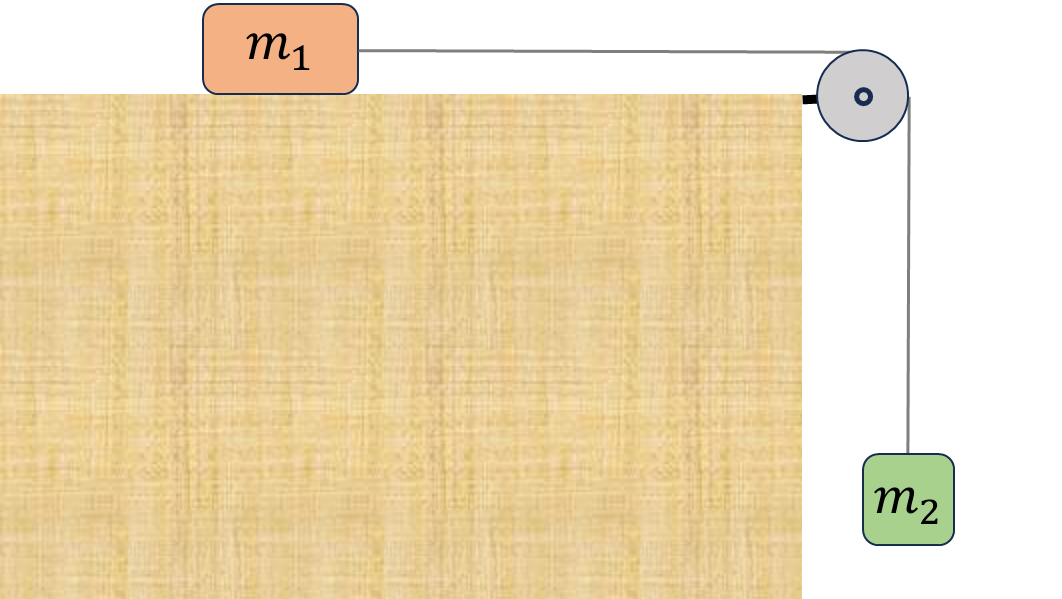
\includegraphics[width=0.4\linewidth]{../figs/VN10-2023-PH-TP021-1}
	\end{center}
	\begin{enumerate}[label=\alph*)]
		\item Bỏ qua ma sát giữa vật $m_1$ và mặt phẳng ngang.
		\item Hệ số ma sát giữa vật $m_1$ và mặt phẳng ngang là $0,2$.
	\end{enumerate}
}
{\hide{
\begin{enumerate}[label=\alph*)]
	\item Bỏ qua ma sát giữa vật $m_1$ và mặt phẳng ngang.\\
	Phân tích các lực tác dụng lên 2 vật
	\begin{center}
		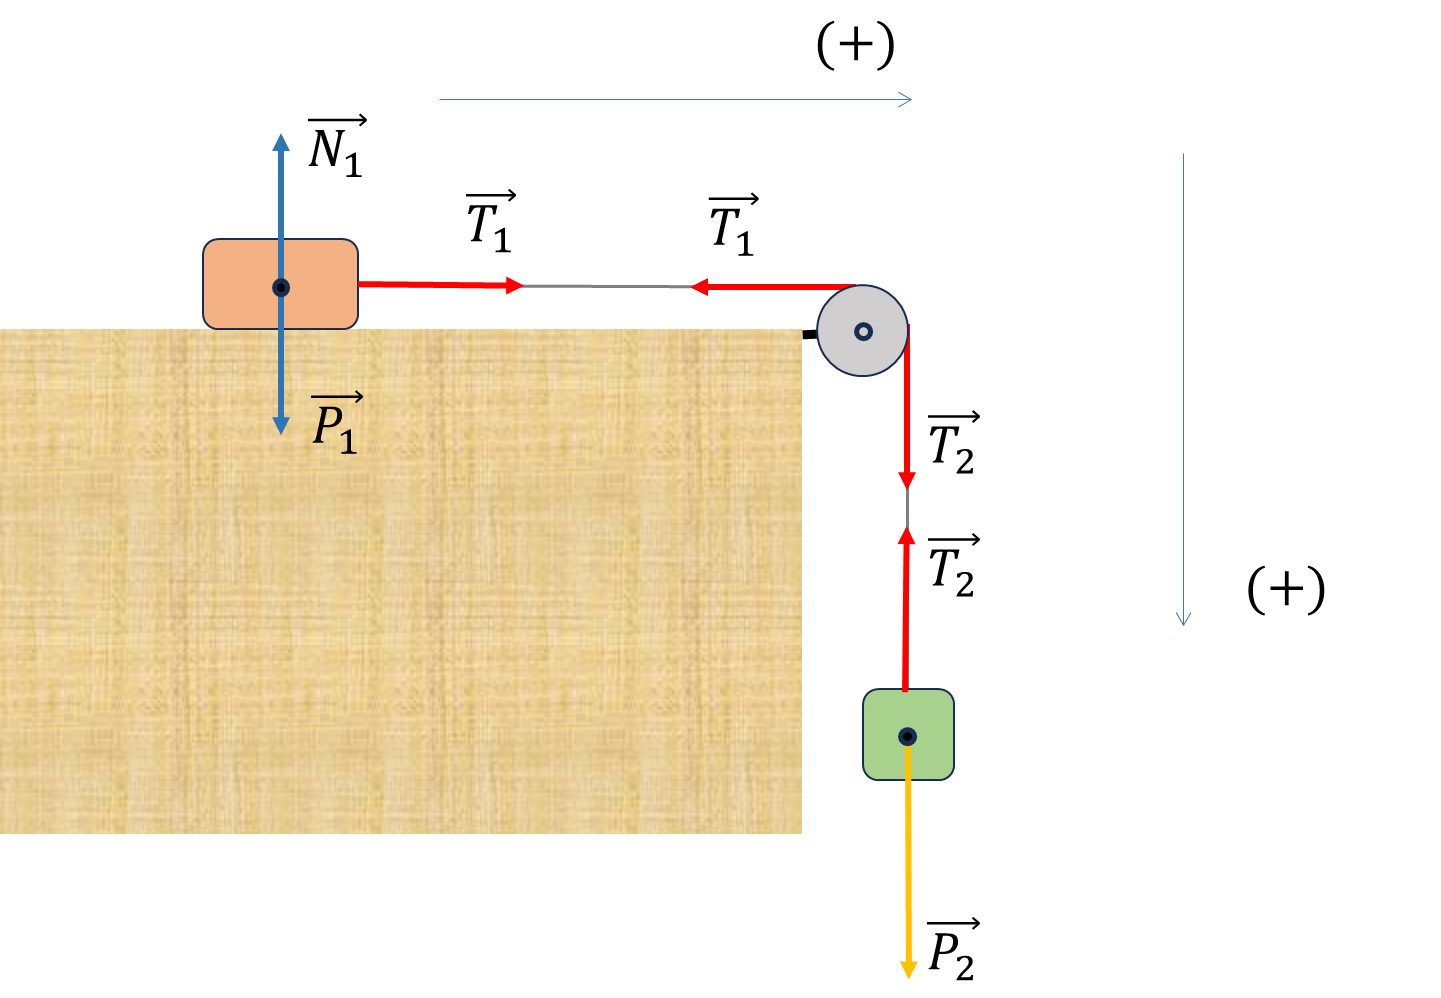
\includegraphics[width=0.6\linewidth]{../figs/VN10-2023-PH-TP021-2}
	\end{center}
Áp dụng định luật II Newton cho mỗi vật:
\begin{itemize}
	\item Vật 1:
	\begin{equation}
		\label{eq:1}
		\overrightarrow{P_1}+\overrightarrow{N_1}+\overrightarrow{T_1}=m_1\overrightarrow{a_1}
	\end{equation}
	\item Vật 2:
	\begin{equation}
		\label{eq:2}
		\overrightarrow{P_2}+\overrightarrow{T_2}=m_2\overrightarrow{a_2}
	\end{equation}
\end{itemize}
Chọn chiều dương như hình vẽ.\\
Lần lượt chiếu phương trình (\ref{eq:1}) và (\ref{eq:2}) lên chiều dương, ta thu được:
\begin{equation}
	\label{eq:3}
	T_1=m_1a_1
\end{equation}
và
\begin{equation}
	\label{eq:4}
	P_2-T_2=m_2a_2
\end{equation}
Vì dây không dãn và bỏ qua khối lượng của ròng rọc nên
$$\begin{cases}
	T_1=T_2=T\\
	a_1=a_2=a
\end{cases}$$
Thay vào phương trình (\ref{eq:3}) và (\ref{eq:4}):
\begin{align}
	\label{eq:5}
	\begin{cases}
		T=m_1a\\
		P_2-T=m_2a
	\end{cases}
\end{align}
$$\Rightarrow P_2=\left(m_1+m_2\right)\cdot a$$
\begin{equation}
	\label{eq:6}
	\Rightarrow a=\dfrac{m_2g}{m_1+m_2}=\dfrac{\left(\SI{4}{\kilogram}\right)\cdot\left(\SI{10}{\meter/\second^2}\right)}{\left(\SI{6}{\kilogram}\right)+\left(\SI{4}{\kilogram}\right)}=\SI{4}{\meter/\second^2}
\end{equation}
Thay phương trình (\ref{eq:6}) vào phương trình (\ref{eq:3}), ta xác định được lực căng dây:
$$T=m_1a=\left(\SI{6}{\kilogram}\right)\cdot\left(\SI{4}{\meter/\second^2}\right)=\SI{24}{\newton}$$
Quãng đường mỗi vật đi được sau 1 giây:
$$s=\dfrac{1}{2}at^2=\dfrac{1}{2}\cdot\left(\SI{4}{\meter/\second^2}\right)\cdot\left(\SI{1}{\second}\right)^2=\SI{2}{\meter}$$
Lực nén lên trục ròng rọc:
$$\overrightarrow{Q}=\overrightarrow{T_1}+\overrightarrow{T_2}$$
$$\Rightarrow Q=\sqrt{T^2_1+T^2_2}=T\sqrt{2}=\xsi{24\sqrt{2}}{\newton}.$$
\item Hệ số ma sát giữa vật $m_1$ và mặt phẳng ngang là $0,2$.\\
Phân tích các lực tác dụng lên 2 vật
\begin{center}
	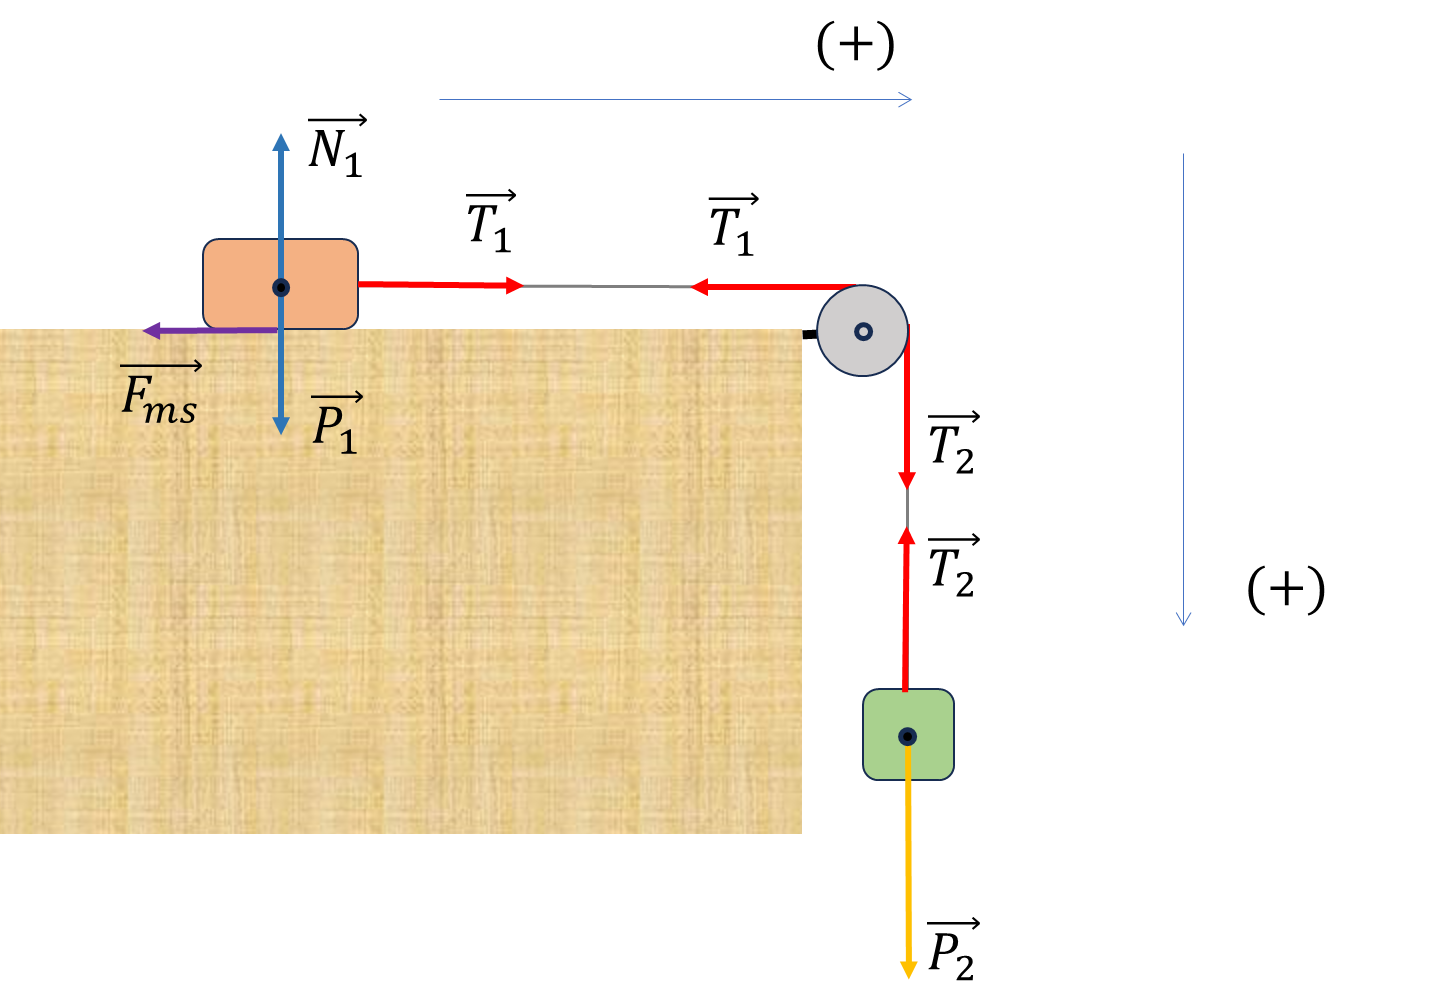
\includegraphics[width=0.6\linewidth]{../figs/VN10-2023-PH-TP021-3}
\end{center}
Áp dụng định luật II Newton cho mỗi vật:
\begin{itemize}
	\item Vật 1:
	\begin{equation}
		\label{eq:7}
		\overrightarrow{P_1}+\overrightarrow{N_1}+\overrightarrow{T_1}+\overrightarrow{F_{ms}}=m_1\overrightarrow{a_1}
	\end{equation}
	\item Vật 2:
	\begin{equation}
		\label{eq:8}
		\overrightarrow{P_2}+\overrightarrow{T_2}=m_2\overrightarrow{a_2}
	\end{equation}
\end{itemize}
Chọn chiều dương như hình vẽ.\\
Lần lượt chiếu phương trình (\ref{eq:1}) và (\ref{eq:2}) lên chiều dương, ta thu được:
\begin{equation}
	\label{eq:9}
	T_1-F_{ms}=m_1a_1
\end{equation}
và
\begin{equation}
	\label{eq:10}
	P_2-T_2=m_2a_2
\end{equation}
Vì dây không dãn và bỏ qua khối lượng của ròng rọc nên
$$\begin{cases}
	T_1=T_2=T\\
	a_1=a_2=a
\end{cases}$$
Thay vào phương trình (\ref{eq:9}) và (\ref{eq:10}):
\begin{align}
	\label{eq:11}
	\begin{cases}
		T-F_{ms}=m_1a\\
		P_2-T=m_2a
	\end{cases}
\end{align}
$$\Rightarrow P_2-F_{ms}=\left(m_1+m_2\right)\cdot a$$
$$\Leftrightarrow m_2g-\mu m_1g=\left(m_1+m_2\right)\cdot a$$
\begin{equation}
	\label{eq:12}
	\Rightarrow a=\dfrac{\left(m_2-\mu m_1\right)g}{m_1+m_2}=\dfrac{\left[\left(\SI{4}{\kilogram}\right)-0,2\cdot\left(\SI{6}{\kilogram}\right)\right]\cdot\left(\SI{10}{\meter/\second^2}\right)}{\left(\SI{6}{\kilogram}\right)+\left(\SI{4}{\kilogram}\right)}=\SI{2.8}{\meter/\second^2}
\end{equation}
Thay phương trình (\ref{eq:12}) vào phương trình (\ref{eq:10}), ta xác định được lực căng dây:
$$T=m_2\cdot\left(g-a\right)=\left(\SI{4}{\kilogram}\right)\cdot\left[\left(\SI{10}{\meter/\second^2}\right)-\left(\SI{2.8}{\meter/\second^2}\right)\right]=\SI{28.8}{\newton}$$
Quãng đường mỗi vật đi được sau 1 giây:
$$s=\dfrac{1}{2}at^2=\dfrac{1}{2}\cdot\left(\SI{2.8}{\meter/\second^2}\right)\cdot\left(\SI{1}{\second}\right)^2=\SI{1.4}{\meter}$$
Lực nén lên trục ròng rọc:
$$\overrightarrow{Q}=\overrightarrow{T_1}+\overrightarrow{T_2}$$
$$\Rightarrow Q=\sqrt{T^2_1+T^2_2}=T\sqrt{2}=\xsi{\dfrac{144\sqrt{2}}{5}}{\newton}.$$
\end{enumerate}
}}
\end{dang}
\begin{dang}{Giải bài toán hệ vật liên kết dây bằng việc xét chuyển động của cả hệ}
	\ppgiai{
	\begin{itemize}
		\item Lực tương tác giữa các vật trong hệ gọi là \textbf{nội lực}. Nội lực không gây ra gia tốc cho toàn hệ.
		\item Lực do yếu tố bên ngoài tác dụng lên hệ gọi là \textbf{ngoại lực}. Nếu các vật của hệ có cùng gia tốc thì 
		$$\sum\overrightarrow{F_\text{ngoài}}=\left(\sum m\right)\cdot\vec{a}$$
	\end{itemize}
}
Ta giải lại các bài ví dụ ở Mục tiêu 2 bằng cách xét chuyển động của cả hệ
\viduii{4}{Hai vật 1 và 2 có thể trượt trên mặt bàn nằm ngang và được nối với nhau bằng dây không dãn, khối lượng dây không đáng kể. Khối lượng của các vật là $m_1 = \SI{2}{kg}$, $m_2=\SI{1}{kg}$. Tác dụng vào vật 1 lực $F=\SI{9}{N}$ theo phương song song với mặt bàn. Hệ số ma sát giữa hai vật với mặt bàn là $\mu=\SI{0.2}{}$. Lấy $g=\SI{10}{m/s^2}$. Hãy tính gia tốc chuyển động của các vật.
}
{\hide{
	\begin{center}
		\begin{tikzpicture}
			\node[anchor=south west,inner sep=0] at (0,0) {\includegraphics[scale=0.7]{G10-17-2}};
			\draw[red,thick,-stealth] (6.8,1.35) -- (5.9,1.35);
			\node[below] at (5.9,1.35) {$\vec{\text{F}}_{\text{ms}_1}$};
		\end{tikzpicture}
		%	\includegraphics[scale=0.5]{../figs/G10-17-2}
	\end{center}
	Vì dây không dãn nên hai vật chuyển động với cùng gia tốc.
	\begin{itemize}
		\item Nội lực của hệ hai vật là lực căng dây: $\overrightarrow{T_1}$ và $\overrightarrow{T_2}$.
		\item Ngoại lực tác dụng lên hệ gồm: $\overrightarrow{P_2}$, $\overrightarrow{N_2}$, $\overrightarrow{F_{ms2}}$, $\overrightarrow{P_1}$, $\overrightarrow{N_1}$, $\overrightarrow{F_{ms1}}$ và $\overrightarrow{F}$.
	\end{itemize}
	Áp dụng định luật II Newton cho cả hệ:
	\begin{equation}
		\label{eq:14}
		\overrightarrow{F}+\overrightarrow{P_1}+\overrightarrow{N_1}+\overrightarrow{F_{ms1}}+\overrightarrow{P_2}+\overrightarrow{N_2}+\overrightarrow{F_{ms2}}=\left(m_1+m_2\right)\vec{a}
	\end{equation}
Chiếu phương trình (\ref{eq:14}) lên hướng của $\overrightarrow{F}$:
$$F-F_{ms1}-F_{ms2}=\left(m_1+m_2\right)a$$
$$\Rightarrow a=\dfrac{F-\mu\left(m_1+m_2\right)g}{m_1+m_2}=\SI{1}{\meter/\second^2}.$$
}}

\viduii{4}
{Hai vật nhỏ có khối lượng $m_1=\SI{6}{\kilogram}$ và $m_2=\SI{4}{\kilogram}$ được nối với nhau bằng sợi dây nhẹ không dãn vắt qua ròng rọc cố định như hình vẽ. Bỏ qua ma sát giữa dây và ròng rọc, lấy gia tốc trọng trường $g=\SI{10}{\meter/\second^2}$. Ròng rọc có khối lượng không đáng kể. Tìm quãng đường mỗi vật đi được sau khi bắt đầu chuyển động 1 giây và lực nén lên trục ròng rọc trong các trường hợp sau:
	\begin{center}
		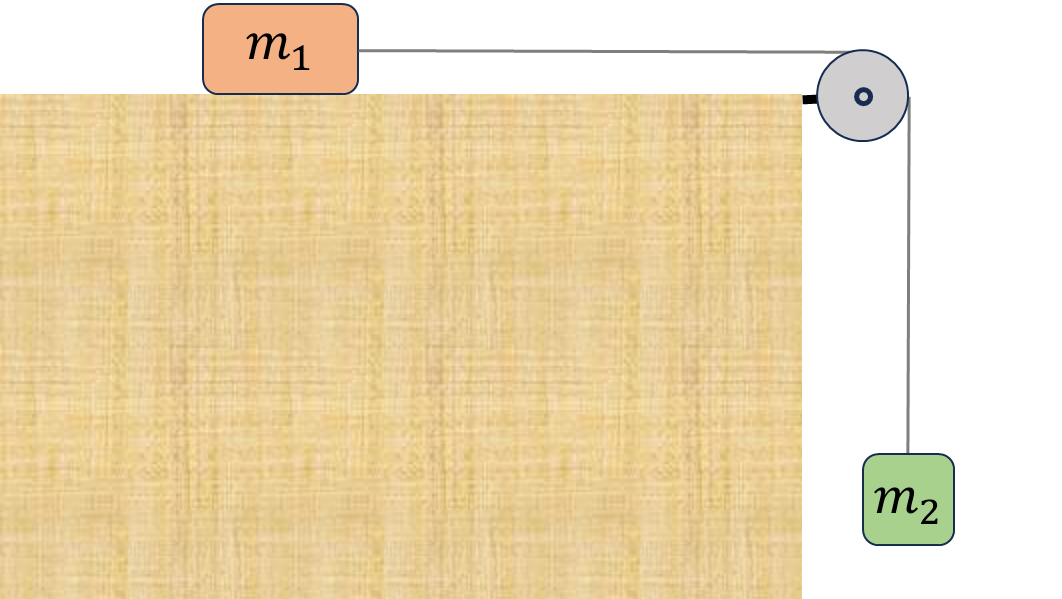
\includegraphics[width=0.4\linewidth]{../figs/VN10-2023-PH-TP021-1}
	\end{center}
	\begin{enumerate}[label=\alph*)]
		\item Bỏ qua ma sát giữa vật $m_1$ và mặt phẳng ngang.
		\item Hệ số ma sát giữa vật $m_1$ và mặt phẳng ngang là $0,2$.
	\end{enumerate}
}
{\hide{
Vì dây không dãn và khối lượng ròng rọc không đáng kể nên hai vật chuyển động cùng gia tốc.
	\begin{enumerate}[label=\alph*)]
		\item Bỏ qua ma sát giữa vật $m_1$ và mặt phẳng ngang.\\
		Phân tích các lực tác dụng lên 2 vật
		\begin{center}
			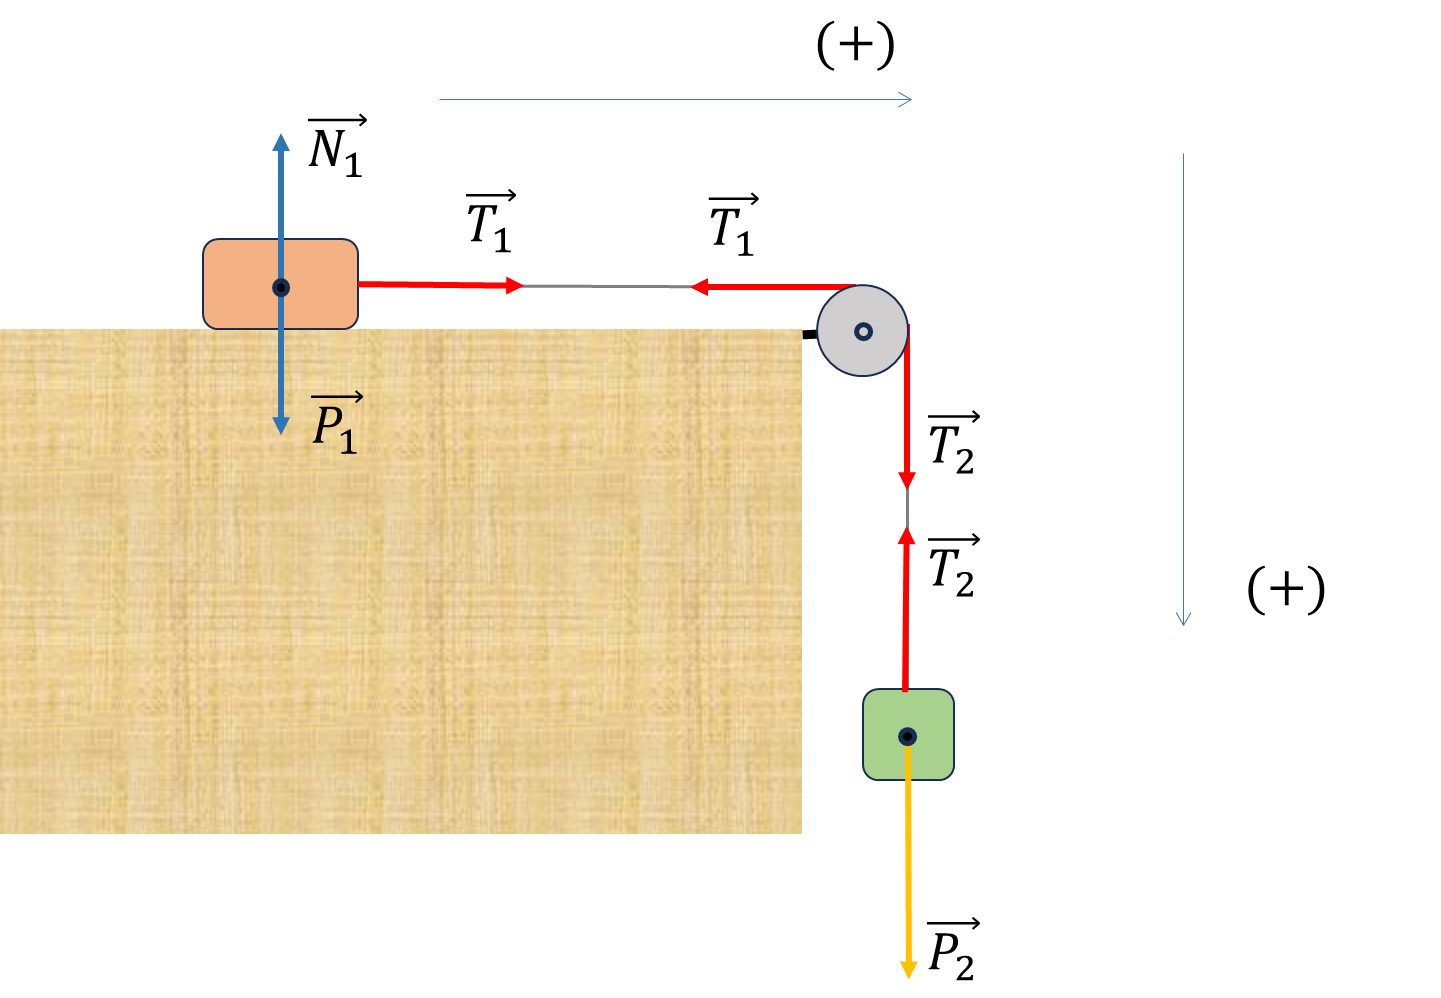
\includegraphics[width=0.6\linewidth]{../figs/VN10-2023-PH-TP021-2}
		\end{center}
		\begin{itemize}
			\item Nội lực gồm: Lực căng dây $\overrightarrow{T_1}$ và $\overrightarrow{T_2}$.
			\item Ngoại lực tác dụng lên hệ gồm: $\overrightarrow{P_1}$, $\overrightarrow{N_1}$ và $\overrightarrow{P_2}$.
		\end{itemize}
	Áp dụng định luật II Newton cho cả hệ:
	\begin{equation}
		\label{eq:15}
		\overrightarrow{P_2}+\overrightarrow{P_1}+\overrightarrow{N_1}=\left(m_1+m_2\right)\vec{a}
	\end{equation} 
	Chiếu phương trình (\ref{eq:15}) lên chiều dương:
	$$P_2=\left(m_1+m_2\right)a \Rightarrow a=\dfrac{m_2g}{m_1+m_2}=\SI{4}{\meter/\second^2}$$
	Xét chuyển động của vật 1, lực căng dây:
	$$T_1=m_1a=\SI{2.4}{\newton}$$
	Quãng đường mỗi vật đi được sau 1 giây:
	$$s=\dfrac{1}{2}at^2=\dfrac{1}{2}\cdot\left(\SI{4}{\meter/\second^2}\right)\cdot\left(\SI{1}{\second}\right)^2=\SI{2}{\meter}$$
	Lực nén lên trục ròng rọc:
	$$\overrightarrow{Q}=\overrightarrow{T_1}+\overrightarrow{T_2}$$
	$$\Rightarrow Q=\sqrt{T^2_1+T^2_2}=T\sqrt{2}=\xsi{24\sqrt{2}}{\newton}.$$
		\item Hệ số ma sát giữa vật $m_1$ và mặt phẳng ngang là $0,2$.\\
		Phân tích các lực tác dụng lên 2 vật
		\begin{center}
			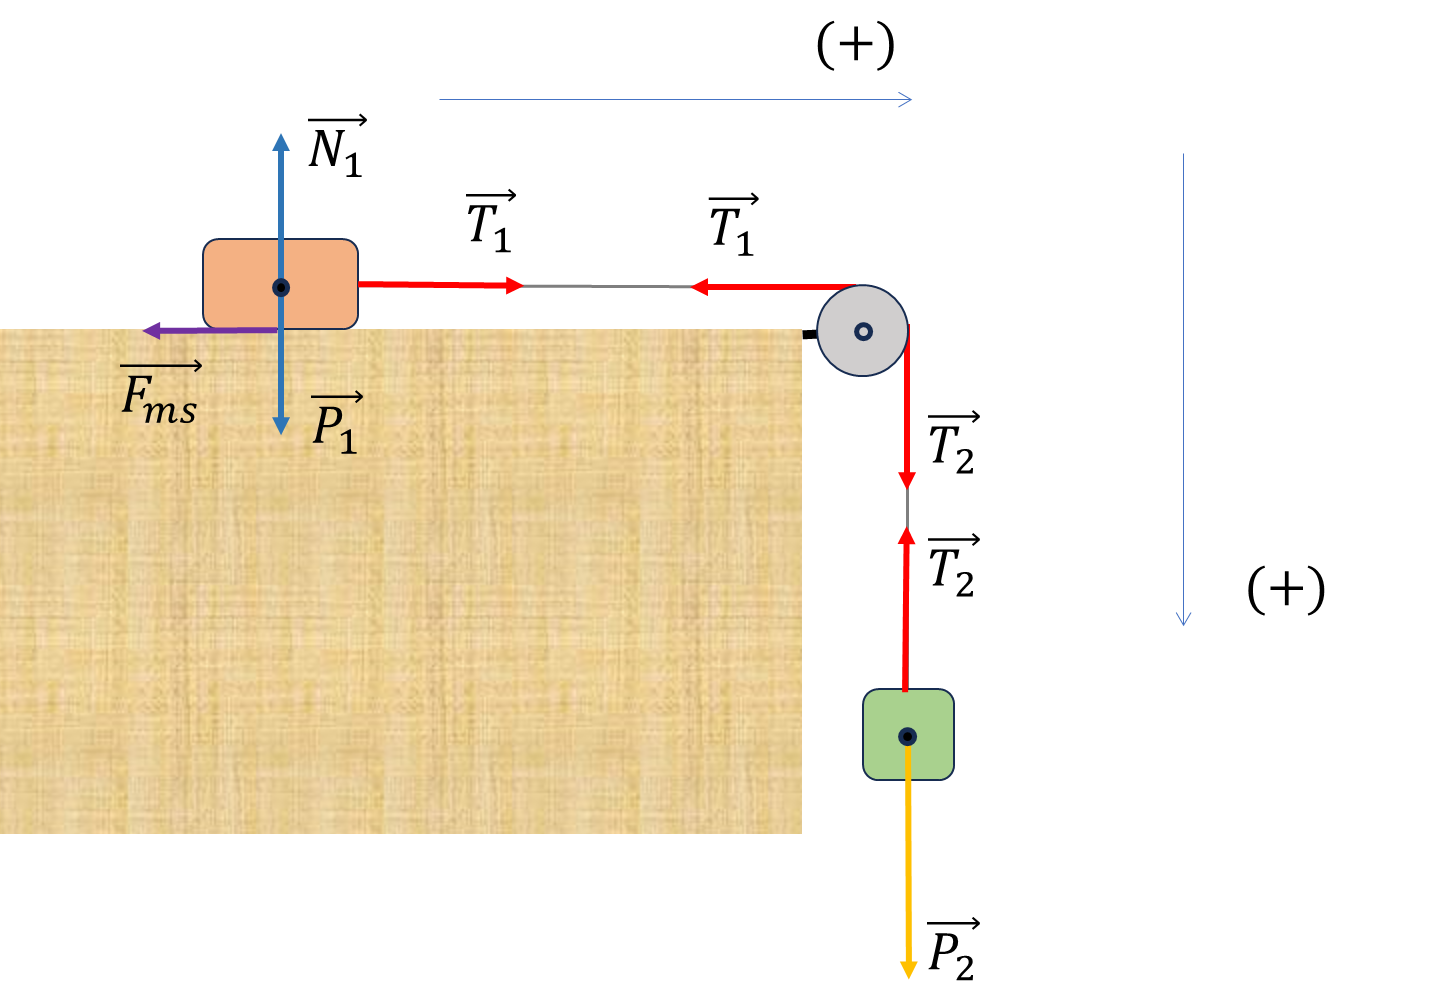
\includegraphics[width=0.6\linewidth]{../figs/VN10-2023-PH-TP021-3}
		\end{center}
		\begin{itemize}
			\item Nội lực gồm: Lực căng dây $\overrightarrow{T_1}$ và $\overrightarrow{T_2}$.
			\item Ngoại lực tác dụng lên hệ gồm: $\overrightarrow{P_1}$, $\overrightarrow{N_1}$, $\overrightarrow{F_{ms}}$ và $\overrightarrow{P_2}$.
		\end{itemize}
		Áp dụng định luật II Newton cho cả hệ:
		\begin{equation}
			\label{eq:16}
			\overrightarrow{P_2}+\overrightarrow{P_1}+\overrightarrow{N_1}+\overrightarrow{F_{ms}}=\left(m_1+m_2\right)\vec{a}
		\end{equation} 
		Chiếu phương trình (\ref{eq:16}) lên chiều dương:
		$$P_2-F_{ms}=\left(m_1+m_2\right)a \Rightarrow a=\dfrac{\left(m_2-\mu m_1\right)g}{m_1+m_2}=\SI{2.8}{\meter/\second^2}$$
		Xét chuyển động của vật 2, xác định được lực căng dây:
		$$T=m_2\cdot\left(g-a\right)=\left(\SI{4}{\kilogram}\right)\cdot\left[\left(\SI{10}{\meter/\second^2}\right)-\left(\SI{2.8}{\meter/\second^2}\right)\right]=\SI{28.8}{\newton}$$
		Quãng đường mỗi vật đi được sau 1 giây:
		$$s=\dfrac{1}{2}at^2=\dfrac{1}{2}\cdot\left(\SI{2.8}{\meter/\second^2}\right)\cdot\left(\SI{1}{\second}\right)^2=\SI{1.4}{\meter}$$
		Lực nén lên trục ròng rọc:
		$$\overrightarrow{Q}=\overrightarrow{T_1}+\overrightarrow{T_2}$$
		$$\Rightarrow Q=\sqrt{T^2_1+T^2_2}=T\sqrt{2}=\xsi{\dfrac{144\sqrt{2}}{5}}{\newton}.$$
	\end{enumerate}
}}
\end{dang}

